\documentclass[final]{article}
\usepackage{neurips_2023}

\usepackage[utf8]{inputenc} % allow utf-8 input
\usepackage[T1]{fontenc}    % use 8-bit T1 fonts
\usepackage{hyperref}       % hyperlinks
\usepackage{url}            % simple URL typesetting
\usepackage{booktabs}       % professional-quality tables
\usepackage{amsfonts}       % blackboard math symbols
\usepackage{nicefrac}       % compact symbols for 1/2, etc.
\usepackage{microtype}      % microtypography
\usepackage{xcolor}         % colors

\usepackage{graphicx}       % For image
\usepackage{float}          % For image H option
\usepackage{enumitem}       % For enumerate
\usepackage{bm}             % For bold math symbols
\usepackage{subcaption}     % For subfigures
\usepackage{amsmath}        % For math symbols

\title{Segmentation of Vessels in Retinal Images}

\author{%
    Shiyu Wang \\
    M.S. in Computational Biology \\
    Carnegie Mellon University \\
    Pittsburgh, PA 15213 \\
    \texttt{shiyuwa2@andrew.cmu.edu} \\
    \And
    Enhao He \\
    M.S. in Computational Biology \\
    Carnegie Mellon University \\
    Pittsburgh, PA 15213 \\
    \texttt{enhaoh@andrew.cmu.edu} \\
    \AND
    Jiacheng Ma \\
    M.S. in Computational Biology \\
    Carnegie Mellon University \\
    Pittsburgh, PA 15213 \\
    \texttt{jiachenm@andrew.cmu.edu} \\
    \And
    Joe Wang \\
    M.S. in Computational Biology \\
    Carnegie Mellon University \\
    Pittsburgh, PA 15213 \\
    \texttt{joewang@andrew.cmu.edu} \\
}


\begin{document}

\maketitle

\vspace{-0.5cm}

\section{Introduction}
\textbf{Problem Statement.} Retinal vessel segmentation is a critical task in medical image analysis that involves isolating the blood vessels from retinal images. Despite its importance in diagnosing ocular diseases, such as diabetic retinopathy and glaucoma \citep{1}, accurate segmentation remains challenging for machine learning methods due to the complex vessel structures, low contrast between the vessels and the surrounding tissue, and varying illumination conditions. \\
\textbf{Motivation.} The motivation for this work stems from the need to enhance early diagnosis and treatment of retinal disorders. Precise vessel segmentation provides key geometric information—such as blood vessel width and tortuosity—that can be correlated with disease progression \citep{review2022}. Automating this process not only accelerates clinical assessments but also reduces the variability and subjectivity inherent in manual segmentation methods, thereby potentially improving patient outcomes. \\
\textbf{Overview of Methods.} In this work, we evaluate four machine learning methods for retinal vessel segmentation. Our approach includes a \textbf{K-means clustering} algorithm that groups pixels based on intensity and color features with contrast enhancement; a \textbf{Naive Bayes Classifier} that uses intensity and gradient information to probabilistically differentiate vessel from non-vessel pixels; a \textbf{Support Vector Machine (SVM)} that finds an optimal hyperplane using pixel-wise features and both linear and non-linear kernels; and a \textbf{Random Forest Classifier} that leverages texture and edge features through an ensemble of decision trees. Together, these methods provide complementary strengths to effectively tackle the segmentation challenge. \\
% In this work, we propose to implement and evaluate four machine learning methods to achieve retinal vessel segmentation. First, we adopt a \textbf{K-means clustering} approach—an unsupervised algorithm that groups pixels based on intensity and color features, enhanced by preprocessing techniques such as contrast enhancement to improve the separation of vessel and non-vessel regions. Complementing this, a \textbf{Naive Bayes Classifier} is employed as a probabilistic model that leverages Bayes' theorem under the assumption of feature independence, and it is trained on manually segmented images to capture the probability distributions of vessel and non-vessel pixels using features like intensity and gradient information. In addition, a \textbf{Support Vector Machine (SVM)} is applied as a supervised learning method that identifies an optimal hyperplane to separate classes by using extracted pixel-wise features, such as intensity and local contrast, with both linear and non-linear kernels to enhance vessel-background discrimination. Finally, a \textbf{Random Forest Classifier} is implemented as an ensemble learning method that constructs multiple decision trees and utilizes features including texture and edge information, thereby boosting segmentation robustness and accuracy through feature importance integration and majority voting. Together, these methods offer complementary strengths to effectively tackle the challenges of accurately segmenting retinal vessels.
\textbf{Dataset.} The experimental analysis is performed on the DRIVE (Digital Retinal Images for Vessel Extraction) dataset, which is widely recognized in the research community for retinal image analysis. The dataset includes high-resolution retinal images along with manually annotated vessel masks, offering a challenging benchmark due to issues like uneven illumination and the subtle contrast between vessels and the background.



\section{Data}
The DRIVE database comprises a total of 40 high-resolution retinal photographs originally obtained from a diabetic retinopathy screening program in The Netherlands. Each image was acquired with a 45° field of view and is stored as an 8-bit per color plane JPEG file at a resolution of 768 by 584 pixels, with a circular field of view of approximately 540 pixels in diameter. The dataset is evenly divided into a training set and a test set, each containing 20 images. \\
Since expert ophthalmologists have provided manual segmentations of the vasculature for the \textbf{training set}, we only use these \textbf{20 images} for training and evaluation. Based on the professional manual segmentations, each pixel's intensity value can be used not only for segmentation but also for extracting key morphological features such as vessel length, width, tortuosity, branching patterns, and angles. These continuous features offer detailed insight into the anatomical and pathological characteristics of the retinal vessels, enabling comparative studies on segmentation performance as well as applications in disease diagnosis, screening, and even biometric identification.



\section{Methods}
The overall \textbf{methodology} is implemented in \texttt{python} and consists of multiple stages including data loading, preprocessing, classification, optimization, and evaluation. \\
As for the \textbf{model} used, we mainly focus on the machine learning model, including K-means Clustering, Naive Bayes Classifier, Support Vector Machine and Random Forest Classifier. \\
To comprehensively \textbf{evaluate} our methods, we will use several metrics including accuracy, sensitivity, specificity, F1-score, and the area under the ROC curve (AUC).
\subsection{Data Loading and Preprocessing}
The DRIVE dataset is loaded by reading the retinal images, manually segmented vessel masks, and background mask data using libraries such as \texttt{tifffile}, \texttt{PIL}, and \texttt{numpy}. \\
Preprocessing part mainly focuses on the \textbf{Image Augmentation}. Our multi-stage enhancement pipeline first amplifies color saturation to emphasize blood vessel structures, then adjusts brightness to improve visibility of subtle features, and finally enhances contrast to sharpen the boundaries between vessels and surrounding tissues. \\
Besides, we also remove the background from the original image to focus on the non-background pixels by using the background mask in the dataset. 
\subsection{K-means Clustering}
\textbf{1. Determining the Optimal Cluster Number} \\
According to the structure of normal retinal photographs, the optimal number of clusters should be \textbf{4}, including: macula (dark shadow in the center), optic disc (bright shadow on the side), blood vessels, and others. But in computer's language, more detailed exploration is still needed. \\
\textbf{2. Optimized K-means Algorithm} \\
To address the challenge of correctly identifying vessel clusters, an optimized version of K-means is used. It merges the clusters with higher AUC values and improves the segmentation performance. To match the biological explanation at the beginning of this section, we merge the top 3 clusters with the highest AUC values to form the final vessel segmentation mask (since $10/3 \sim 4$).\\
\textbf{3. Image Augmentation with Optimized K-means} \\
Image augmentation was further applied to enhance the quality of vessel segmentation. By pre-enhancing the input images, the clustering algorithm produces improved segmentation results. \\
\textbf{4. Direction-enhanced K-means Clustering} \\
To further improve segmentation, we try to utilize the fact that blood vessels are long and thin by incorporating the \textbf{gradient-based features} into the clustering process. In this approach, the original RGB features are augmented with gradient magnitude and gradient direction (obtained via the Sobel filter), forming an enhanced feature vector. Such directional information helps to better delineate vessel boundaries.
\subsection{Random Forest Classification}
The random forest algorithm, a robust ensemble learning method, can be effectively applied to retinal image segmentation by leveraging its ability to classify pixels into anatomical or pathological regions through supervised learning. In this context, features such as pixel intensity, texture gradients, local binary patterns, and responses to edge-detection filters (e.g., Sobel or Gabor) are extracted from retinal images to capture structural details of blood vessels, lesions, or the optic disc. During training, the algorithm constructs multiple decision trees, each trained on random subsets of the data and features, to predict pixel-wise labels from annotated ground-truth masks. At inference, the ensemble aggregates predictions across trees, assigning each pixel to the most probable class (e.g., vessel vs. non-vessel), while mitigating overfitting through majority voting. 
\paragraph{Training Process:} The gist of Random Forest is to build multiple decision trees and aggregate their predictions. The training process involves the following steps: 
\begin{enumerate}
    \item \textbf{Feature Extraction}: Extract features from the training images, in our cases, the features are simply the RGB values of the pixels.
    \item \textbf{Random Sampling}: Randomly select subsets of the training data and features to build each decision tree, ensuring diversity among trees.
    \item \textbf{Tree Construction}: For each subset, construct a decision tree by recursively splitting the data based on feature thresholds that maximize information gain or minimize Gini impurity (which is the taken approach).
    
\textbf{Gini impurity} (for class \( k \)):  
\[
G = 1 - \sum_{k=1}^K p_k^2
\]  
where \( p_k \) is the proportion of samples of class \( k \) in the node.  

\textbf{Information gain} (using entropy \( H \)):  
\[
H = -\sum_{k=1}^K p_k \log p_k
\]  
\[
\text{Information Gain} = H_{\text{parent}} - \sum_{\text{child}} \frac{N_{\text{child}}}{N_{\text{parent}}} H_{\text{child}}
\]  

    \item \textbf{Prediction Aggregation}: At inference, aggregate predictions from all trees using majority voting to assign the final class label to each pixel.
\end{enumerate}


\section{Results}
\subsection{K-means Clustering}
\subsubsection{Optimal Cluster Number Determination}
After evaluating different numbers of clusters (ranging from 2 to 10) by computing the AUC value for each image and taking the mean value, we found that the AUC value and the details of the vessels are positively correlated with the number of clusters, as shown in the Supplementary Figures ~\ref{fig:nclusters}, ~\ref{fig:n=2}, ~\ref{fig:n=6}, ~\ref{fig:n=10}, and ~\ref{fig:specificcase}. \\
However, when we set the \texttt{n\_clusters} = 10, the vessel pixels are fragmented into multiple clusters. Thus, a single cluster in each image is not sufficient to evaluate the segmentation performance. \\
Therefore, we decided to set \texttt{n\_clusters} = 10 as an optimal compromise with an \textbf{optimized K-means algorithm}.
\subsubsection{Optimized K-means Results}
Figure~\ref{fig:opt1} depict the best segmentation examples using this approach, including the original image, the ground truth, the segmentation result with AUC values, and the segmentation overlay. The second and third best examples are shown in the Supplementary Figures ~\ref{fig:opt2}, and ~\ref{fig:opt3}. 
\begin{figure}[H]
    \centering
    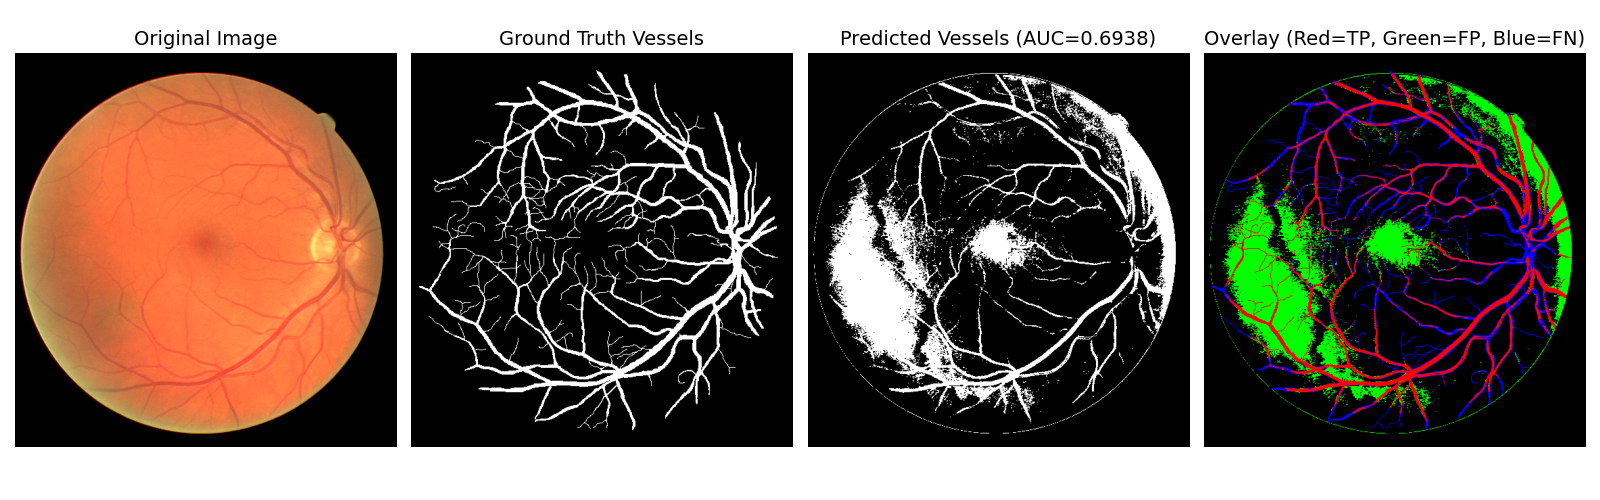
\includegraphics[scale=0.25]{Figures/3 Optimized 1st.png}
    \vspace{-0.25cm}
    \caption{Optimized K-means: the first best example (AUC=0.6938)}
    \label{fig:opt1}
\end{figure}
As we can see, the biggest problem is that there are a lot of false positive pixels (FP, Green) in the segmentation results, which means that their colors are difficult to distinguish from blood vessels. 
\subsubsection{Image Augmentation with Optimized K-means Results}
The results corresponding to the best examples above after applying image augmentation are shown in Figure~\ref{fig:opt_aug1} below. The other two examples are shown in the Supplementary Figures ~\ref{fig:opt_aug2}, and ~\ref{fig:opt_aug3}.
\begin{figure}[H]
    \centering
    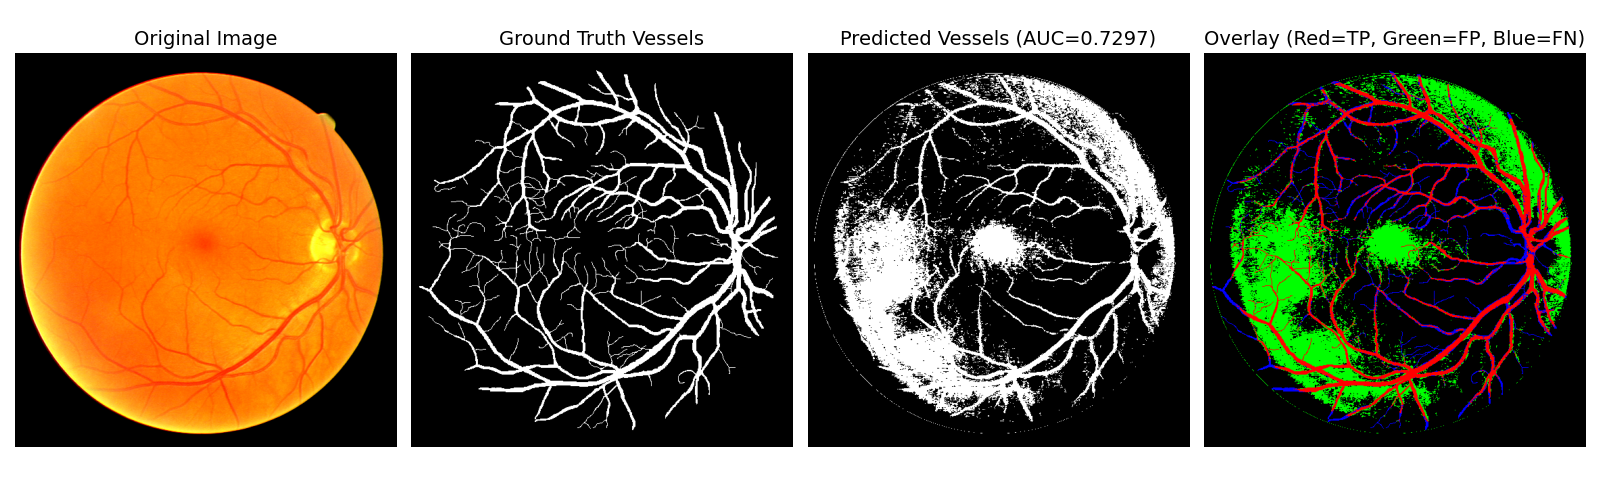
\includegraphics[scale=0.25]{Figures/4 Optimized 1st.png}
    \vspace{-0.25cm}
    \caption{Optimized K-means with augmentation: the first best example (AUC=0.6938 $\rightarrow$ \textcolor{red}{0.7297})}
    \label{fig:opt_aug1}
\end{figure}
Apparently, the results are much better now. The false positive pixels (FP, Green) are significantly reduced, and the segmentation results are more accurate. 
\subsubsection{Direction-enhanced K-means Clustering Results}
Such directional information helps to better delineate vessel boundaries, as illustrated in the following figures (Figure~\ref{fig:de}).
\begin{figure}[H]
    \centering
    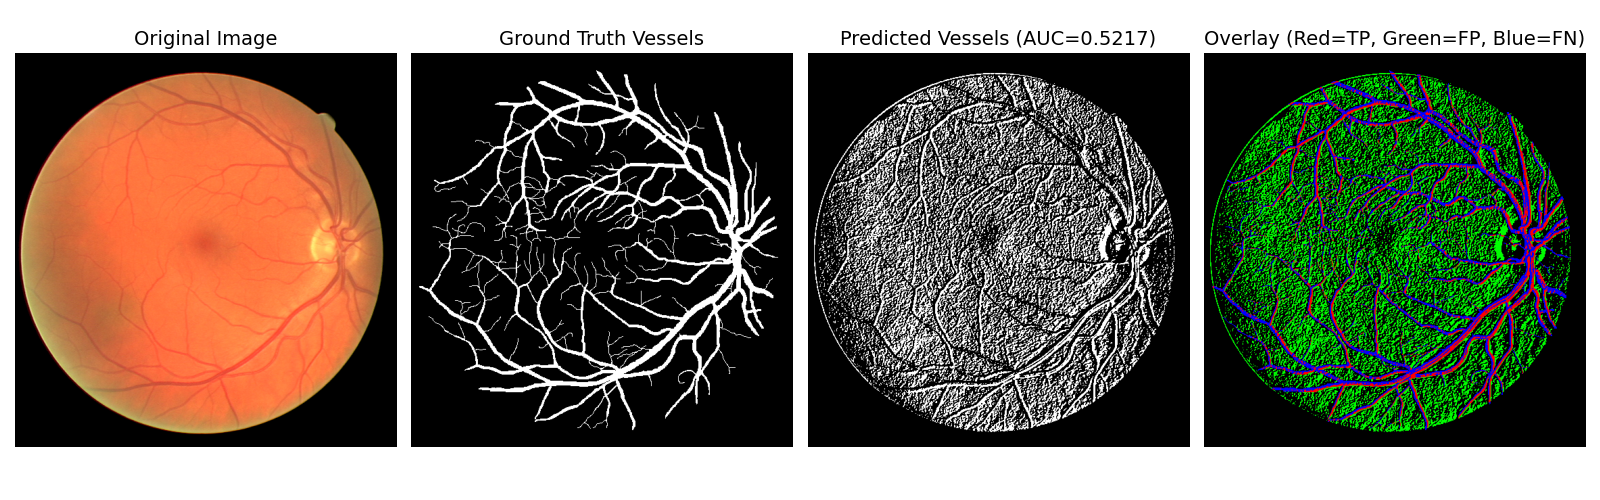
\includegraphics[scale=0.25]{Figures/5 Directed (Merge 3 Clusters).png}
    \vspace{-0.25cm}
    \caption{Direction-enhanced K-means (AUC=0.5217)}
    \label{fig:de}
\end{figure}
The overall performance of the direction-enhanced K-means is not as good as previous methods, but it still provides a different perspective on the segmentation task by showing the potential of incorporating gradient features. Also, the results are in a different style, which is quite interesting. \\
Besides, we can also see the small improvement of the AUC value after applying image augmentation (see Supplementary Figure~\ref{fig:de_aug}), which further verify the effectiveness of this technique. 
\subsubsection{Performance Evaluation and Comparison}
Table~\ref{tab:performance} summarizes the performance comparison between the classic K-means and the optimized K-means methods, both before and after applying image augmentation. (Not include the direction-enhanced K-means is because it is just a try and not the main focus of this project.) 
\begin{table}[H]
    \centering
    \caption{Performance Comparison: Before (Black) and After (Red) Image Augmentation}
    \label{tab:performance}
    \begin{tabular}{lcc}
    \toprule
    \textbf{Metric} & \textbf{Classic K-means} & \textbf{Optimized K-means} \\
    \midrule
    Accuracy & $0.8062 \rightarrow \textcolor{red}{0.8404}$ & $0.6193 \rightarrow \textcolor{red}{0.6938}$ \\
    Sensitivity & $0.2228 \rightarrow \textcolor{red}{0.2805}$ & $0.5862 \rightarrow \textcolor{red}{0.6138}$ \\
    Specificity & $0.8898 \rightarrow \textcolor{red}{0.9200}$ & $0.6247 \rightarrow \textcolor{red}{0.7057}$ \\
    F1 Score   & $0.2270 \rightarrow \textcolor{red}{0.3115}$ & $0.2802 \rightarrow \textcolor{red}{0.3393}$ \\
    AUC value    & $0.5563 \rightarrow \textcolor{red}{0.6003}$ & $0.6054 \rightarrow \textcolor{red}{0.6598}$ \\
    \bottomrule
    \end{tabular}
\end{table}
Through comparison of evaluation metrics, it is evident that image augmentation has a positive impact on both K-means algorithms. \\
Although classic K-means shows better performance in accuracy and specificity, the optimized K-means algorithm demonstrates significant advantages in key metrics such as sensitivity and AUC value, especially when combined with image augmentation techniques, providing more effective discrimination between vessel and non-vessel regions. \\
This suggests that the optimized K-means algorithm has stronger recognition capabilities in vessel segmentation applications, making it particularly suitable for medical image analysis tasks that require higher detection rates.

\subsection{Random Forest Classification}
Through the whole training process, totally 10 images, \(10 \times 584 \times 565 = 3299600\) pixels are trained upon. The pixels are separeted into 3 classes: 0 for masked boundary, 1 for background and 2 for blood vessels. A typical prediction result given by the classifier is shown below in Figure~\ref{fig:mjct27} and Table~\ref{tab:mjct27}, with an AUC of approximately \textbf{0.6176}. 
\begin{figure}[H]
    \centering
        \centering
        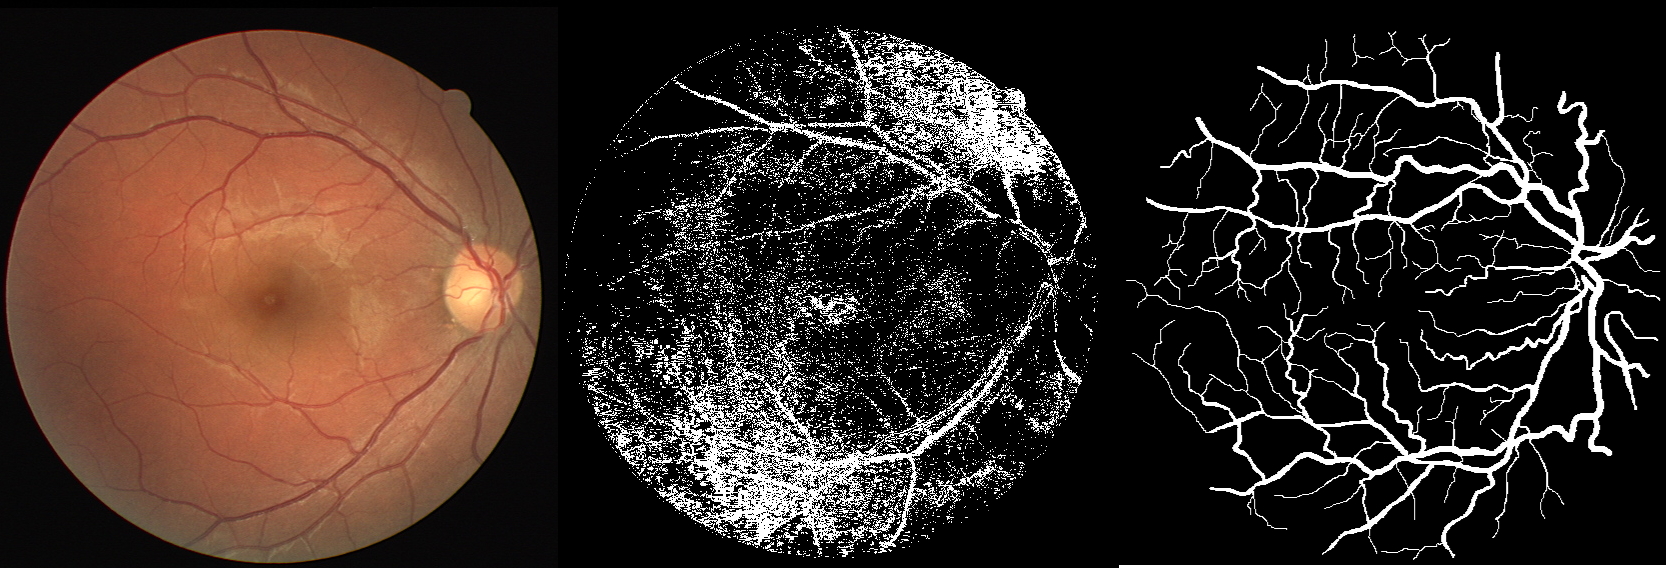
\includegraphics[scale=0.2]{Figures/mjc.png}
        \caption{1st image is the original image, 2nd image is the manually labeled image for training, 3rd image is the predicted image by the random forest algorithm.}\label{fig:mjct27}
\end{figure}
\vspace{-0.75cm}
\begin{table}[H]
    \centering
    \caption{Metrics for the segmentation Task}
    \begin{tabular}{ccccc}
    \toprule
                     & precision & recall & f1-score & support \\
    \midrule
    background       & 0.91      & 0.80 (specificity) & 0.85     & 198755  \\
    retinal          & 0.24      & 0.44 (sensitivity) & 0.31     & 29073   \\
    accuracy         &           &        & 0.75      & 227828  \\
    weighted average & 0.82      & 0.75   & 0.78      & 227828  \\
    \bottomrule
    \end{tabular}
    \label{tab:mjct27}
\end{table}


\section{Discussions}
For this part, we explored classical unsupervised machine learning techniques for retinal vessel segmentation. Through the use of K-means clustering and its optimized variations, including image augmentation and the incorporation of gradient features, the proposed methods demonstrated significant improvements in segmentation performance as measured by standard evaluation metrics. \\
For future work, the following directions are suggested:
\begin{itemize}
    \item \textbf{Improved Image Augmentation:} In addition to traditional geometric transformations (e.g., rotation and flipping), consider advanced photometric adjustments, including saturation, hue, and white balance to mimic different lighting conditions. 
    \item \textbf{Enhanced Feature Extraction:} Incorporating additional features beyond raw RGB values and gradients, such as texture descriptors, fractal-based features, or deep feature representations, to better capture vessel morphology.
\end{itemize}
\newpage











\section{Figures}


\begin{figure}[H]
    \centering
    \fbox{\rule[-.5cm]{0cm}{4cm} \rule[-.5cm]{4cm}{0cm}}
    \caption{Sample figure caption.}
\end{figure}


All artwork must be neat, clean, and legible. Lines should be dark enough for
purposes of reproduction. The figure number and caption always appear after the
figure. Place one line space before the figure caption and one line space after
the figure. The figure caption should be lower case (except for first word and
proper nouns); figures are numbered consecutively.


You may use color figures.  However, it is best for the figure captions and the
paper body to be legible if the paper is printed in either black/white or in
color.


\section{Tables}


All tables must be centered, neat, clean and legible.  The table number and
title always appear before the table.  See Table~\ref{sample-table}.


Place one line space before the table title, one line space after the
table title, and one line space after the table. The table title must
be lower case (except for first word and proper nouns); tables are
numbered consecutively.


Note that publication-quality tables \emph{do not contain vertical rules.} We
strongly suggest the use of the \verb+booktabs+ package, which allows for
typesetting high-quality, professional tables:
\begin{center}
    \url{https://www.ctan.org/pkg/booktabs}
\end{center}
This package was used to typeset Table~\ref{sample-table}.


\begin{table}[H]
    \caption{Sample table title}
    \label{sample-table}
    \centering
    \begin{tabular}{lll}
        \toprule
        \multicolumn{2}{c}{Part}                   \\
        \cmidrule(r){1-2}
        Name     & Description     & Size ($\mu$m) \\
        \midrule
        Dendrite & Input terminal  & $\sim$100     \\
        Axon     & Output terminal & $\sim$10      \\
        Soma     & Cell body       & up to $10^6$  \\
        \bottomrule
    \end{tabular}
\end{table}
\newpage


\section{Author Contributions}
\textbf{Shiyu Wang}: Topic Selection, Proposal, K-means Clustering, Image Augmentation, Final Report. \\
\textbf{Enhao He}: Proposal (methods part), Support Vector Machine, Final Report (SVM related part). \\
\textbf{Jiacheng Ma}: Random Forest Classifier, Final Report (RF related part). \\
\textbf{Joe Wang}: Naive Bayes Classifier, Final Report (NBC related part). \\
The contributions of each author to sildes are equal. 
\newpage


\section{Supplementary Material}
\setcounter{figure}{0}
\renewcommand{\thefigure}{S\arabic{figure}}

% K-means clustering
\begin{figure}[H]
    \centering
    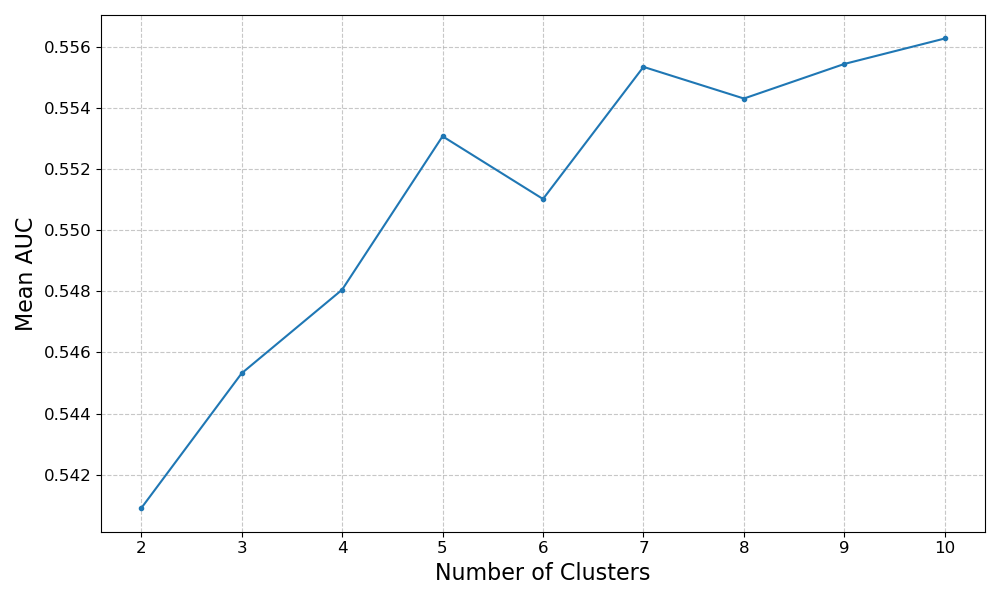
\includegraphics[scale=0.5]{Figures/1-1 Find the Best n_clusters.png}
    \vspace{-0.25cm}
    \caption{Mean AUC values for different number of clusters.}
    \label{fig:nclusters}
\end{figure}
\begin{figure}[H]
    \centering
    \includegraphics[scale=0.3]{Figures/1-2 2 Clusters.png}
    \vspace{-0.25cm}
    \caption{Segmentation results (\texttt{n\_clusters}=2).}
    \label{fig:n=2}
\end{figure}
\begin{figure}[H]
    \centering
    \includegraphics[scale=0.3]{Figures/1-2 6 Clusters.png}
    \vspace{-0.25cm}
    \caption{Segmentation results (\texttt{n\_clusters}=6).}
    \label{fig:n=6}
\end{figure}
\begin{figure}[H]
    \centering
    \includegraphics[scale=0.3]{Figures/1-2 10 Clusters.png}
    \vspace{-0.25cm}
    \caption{Segmentation results (\texttt{n\_clusters}=10).}
    \label{fig:n=10}
\end{figure}
\begin{figure}[H]
    \centering
    \includegraphics[scale=0.5]{Figures/2 10 Clusters.png}
    \vspace{-0.25cm}
    \caption{Specific case (\texttt{n\_clusters}=10).}
    \label{fig:specificcase}
\end{figure}
\begin{figure}[H]
    \centering
    \begin{subfigure}[H]{\textwidth}
        \centering
        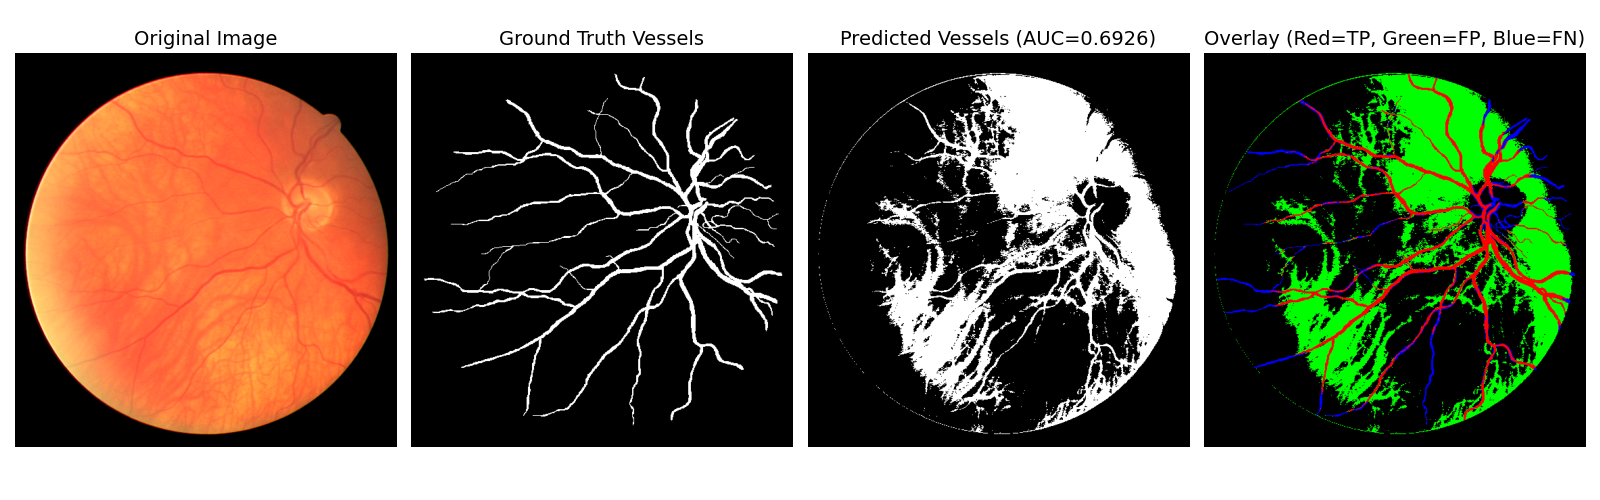
\includegraphics[scale=0.3]{Figures/3 Optimized 2nd.png}
        \vspace{-0.25cm}
        \caption{The second best example (AUC=0.6926)}
        \label{fig:opt2}
    \end{subfigure}
    \begin{subfigure}[H]{\textwidth}
        \centering
        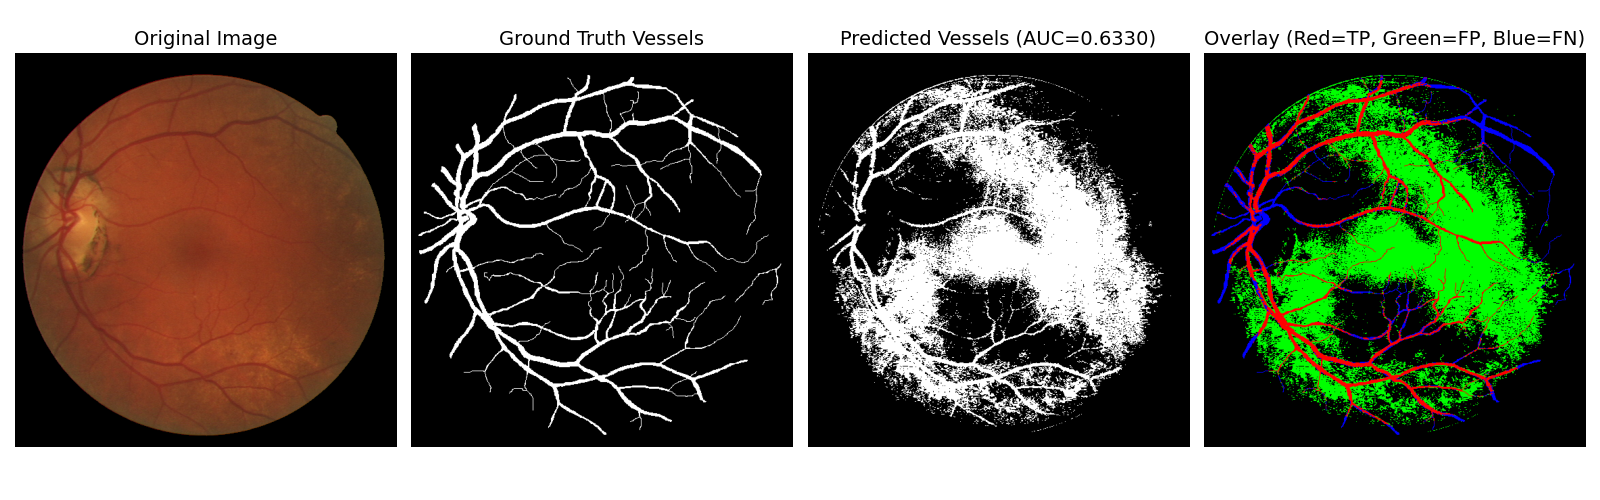
\includegraphics[scale=0.3]{Figures/3 Optimized 3rd.png}
        \vspace{-0.25cm}
        \caption{The third best example (AUC=0.6330)}
        \label{fig:opt3}
    \end{subfigure}
    \caption{Optimized K-means: Top 3 Examples}
    \label{fig:opt}
\end{figure}
\begin{figure}[H]
    \begin{subfigure}[H]{\textwidth}
        \centering
        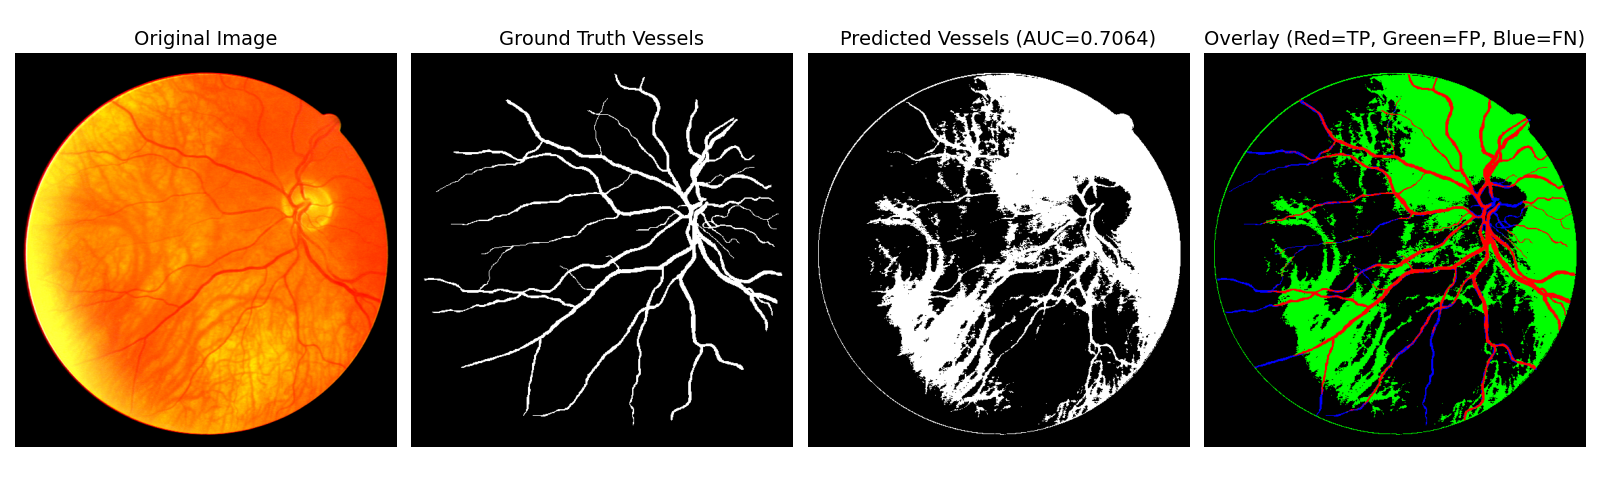
\includegraphics[scale=0.3]{Figures/4 Optimized 2nd.png}
        \vspace{-0.25cm}
        \caption{The second best example (AUC=0.6926 $\rightarrow$ \textcolor{red}{0.7064})}
        \label{fig:opt_aug2}
    \end{subfigure}
\end{figure}
\begin{figure}[H]
    \ContinuedFloat
    \centering
    \begin{subfigure}[H]{\textwidth}
        \centering
        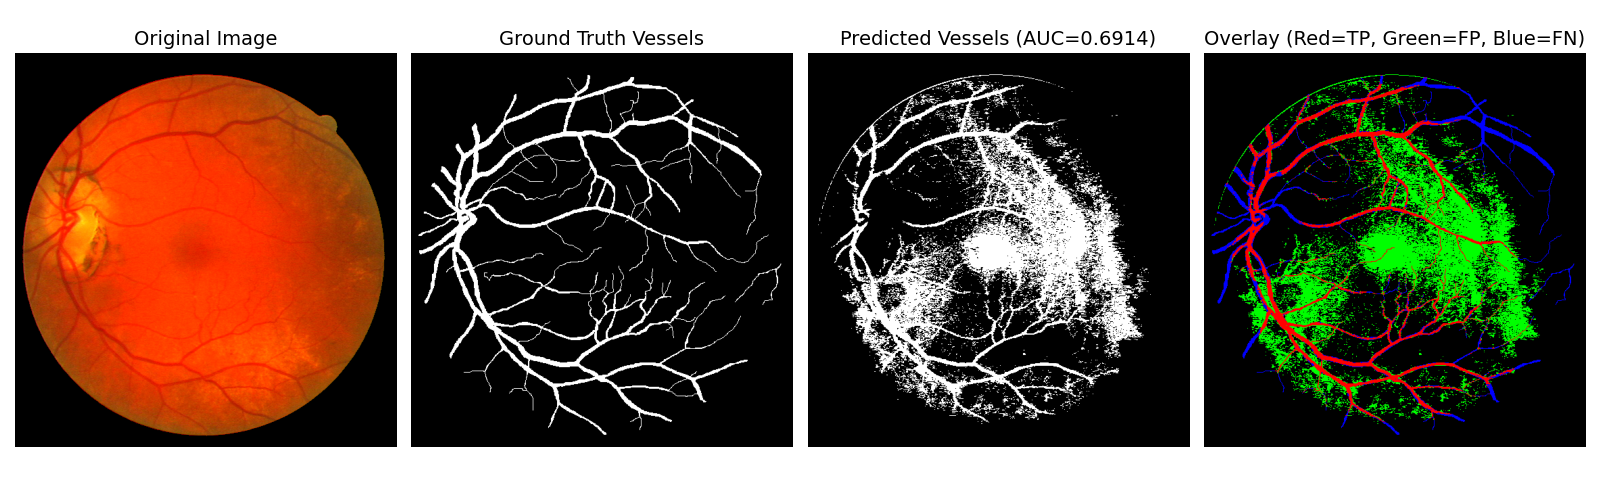
\includegraphics[scale=0.3]{Figures/4 Optimized 3rd.png}
        \vspace{-0.25cm}
        \caption{The third best example (AUC=0.6330 $\rightarrow$ \textcolor{red}{0.6914})}
        \label{fig:opt_aug3}
    \end{subfigure}
    \caption{Optimized K-means with Augmentation: Corresponding 3 Examples}
    \label{fig:opt_aug}
\end{figure}
\begin{figure}[H]
    \centering
    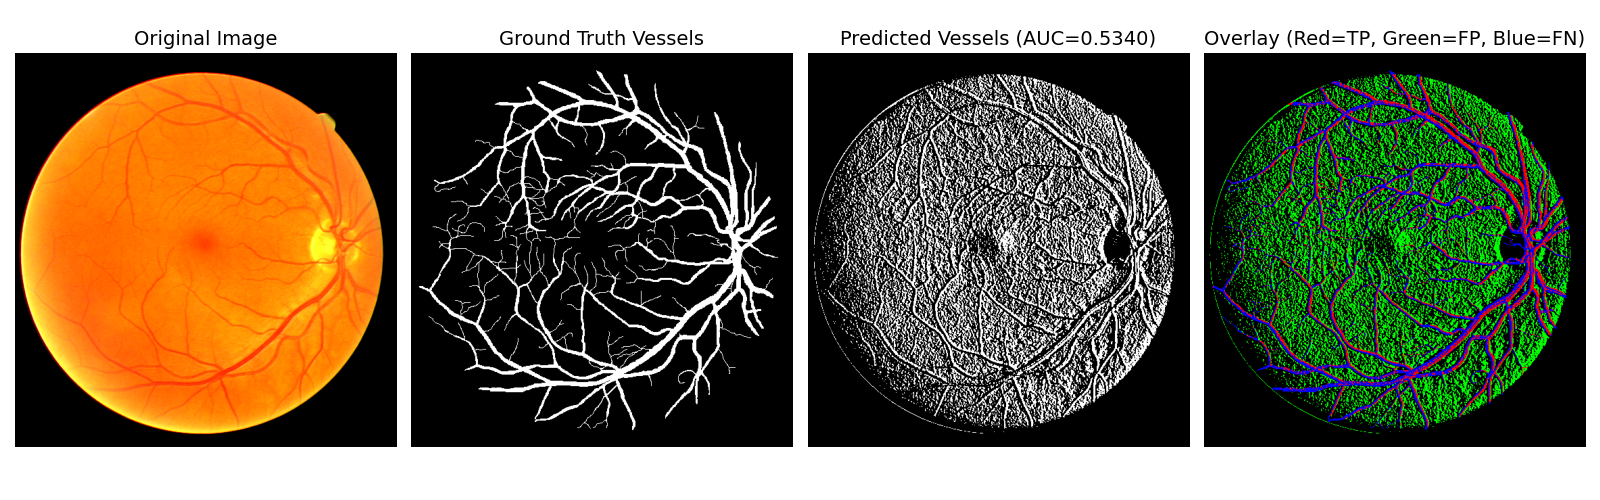
\includegraphics[scale=0.3]{Figures/6 Directed (Merge 3 Clusters).png}
    \vspace{-0.25cm}
    \caption{Direction-enhanced K-means with augmentation (AUC=0.5217 $\rightarrow$ \textcolor{red}{0.5340})}
    \label{fig:de_aug}
\end{figure}






\newpage
\bibliographystyle{unsrtnat}
\bibliography{references}

% \section*{References}
% {
% \small
% [1] Li W, Xiao Y, Hu H, et al. Retinal Vessel Segmentation Based on B-COSFIRE Filters in Fundus Images. Front Public Health. 2022;10:914973. Published 2022 Sep 9. doi:10.3389/fpubh.2022.914973 

% [2] Khandouzi A, Ariafar A, Mashayekhpour Z, Pazira M, Baleghi Y. Retinal Vessel Segmentation, a Review of Classic and Deep Methods. Ann Biomed Eng. 2022;50(10):1292-1314. doi:10.1007/s10439-022-03058-0 

% [3] Liu Z, Sunar MS, Tan TS, Hitam WHW. Deep learning for retinal vessel segmentation: a systematic review of techniques and applications. Med Biol Eng Comput. Published online February 18, 2025. doi:10.1007/s11517-025-03324-y

% [4] Li Y, Zhang Y, Liu JY, et al. Global Transformer and Dual Local Attention Network via Deep-Shallow Hierarchical Feature Fusion for Retinal Vessel Segmentation. IEEE Trans Cybern. 2023;53(9):5826-5839. doi:10.1109/TCYB.2022.3194099

% [5] Li D, Rahardja S. BSEResU-Net: An attention-based before-activation residual U-Net for retinal vessel segmentation. Comput Methods Programs Biomed. 2021;205:106070. doi:10.1016/j.cmpb.2021.106070

% [6] Liu M, Wang Z, Li H, Wu P, Alsaadi FE, Zeng N. AA-WGAN: Attention augmented Wasserstein generative adversarial network with application to fundus retinal vessel segmentation. Comput Biol Med. 2023;158:106874. doi:10.1016/j.compbiomed.2023.106874
% }


%%%%%%%%%%%%%%%%%%%%%%%%%%%%%%%%%%%%%%%%%%%%%%%%%%%%%%%%%%%%


\end{document}